\documentclass{./../../Latex/teaching_slides}

\usepackage{venndiagram}
\usepackage{tikz}
\usepackage{pgfplots}
\usetikzlibrary{arrows.meta}

\begin{document}

\title{ECON 441 \\ \vspace{0.4em} \normalsize Introduction to Mathematical Economics}
\author{Div Bhagia}
\date{Lecture 9 \\ Multivariable Optimization}

%%%%%%%%%%%%%%
\begin{frame}[noframenumbering, plain]
\maketitle
\end{frame}



%%%%%%%%%%%%%%
\begin{frame}{Global vs Local Extrema}
\centering
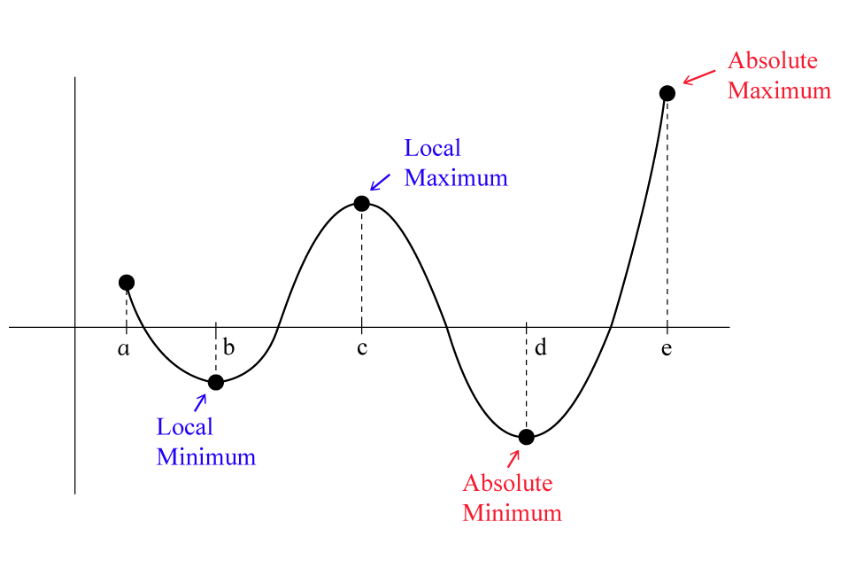
\includegraphics[scale=0.375]{global_vs_local.png}
\end{frame}

%%%%%%%%%%%%%%
\begin{frame}{First-Derivative Test}
\centering
\begin{tikzpicture}[scale=1.25, transform shape]
\begin{axis}[axis lines = center, ymax=3, xtick, ytick, ymin=-2, xmin=-35, xmax=65]
\addplot [domain=-30:60, samples=100, line width = 0.3mm]
{cos(5*x+2)+cos(2*x+2)};
\draw[dashed,red] (250,400) -- (450,400) node[above, yshift=-2, xshift=0] {\scriptsize $f'(x)=0$};
\draw[dashed,red] (650,120) -- (850,120)node[above, yshift=-20, xshift=-12] {\scriptsize $f'(x)=0$};
\node[right, rotate=-60, red] at (480,370) {\scriptsize $f'(x)<0$};
\node[right, rotate=60, red] at (100,255) {\scriptsize $f'(x)>0$};
\node[right, rotate=-30, red] at (480,200) {\scriptsize $f'(x)<0$};
\node[right, rotate=30, red] at (825,120) {\scriptsize $f'(x)>0$};
\end{axis}
\end{tikzpicture}
\end{frame}

%%%%%%%%%%%%%%
\begin{frame}{Necessary vs Sufficient Conds.}
\begin{tabularx}{\textwidth}{lXX}
\hline Condition & Maximum & Minimum \\
\hline \\ 
First-order necessary & $f^{\prime}(x)=0$ & $f^{\prime}(x)=0$ \\~\\
Second-order necessary ${ }^{\dagger}$ & $f^{\prime \prime}(x) \leq 0$ & $f^{\prime \prime}(x) \geq 0$ \\~\\
Second-order sufficient ${ }^{\dagger}$ & $f^{\prime \prime}(x)<0$ & $f^{\prime \prime}(x)>0$ \\~\\
\hline
\end{tabularx}
\vspace{0.25em}

${ }^{\dagger}$ Applicable only after the first-order necessary condition has been satisfied.
\end{frame}

%%%%%%%%%%%%%%
\begin{frame}{Concave and Convex Functions}
\begin{witemize}
  \item Concave function: $ f''(x) \leq 0$ for all $x$ 
  \item Convex function: $ f''(x) \geq 0$ for all $x$ \\~\\
  \item Strictly concave function: $ f''(x) < 0$ for all $x$ 
  \item Strictly convex function: $ f''(x) > 0$ for all $x$ 
\end{witemize}
\end{frame}


%%%%%%%%%%%%%%
\begin{frame}{Global Optimizers}
\begin{witemize}
  \item If a function is concave, any critical point will give us a global maximum.
  \item If a function is strictly concave, any critical point will give us the \textit{unique} global maximum.
  \item If a function is convex, any critical point will give us a global minimum.
  \item If a function is strictly convex, any critical point will give us the \textit{unique} global minimum.
\end{witemize}
\end{frame}

%%%%%%%%%%%%%%
\begin{frame}{Example}
$$ y = 3x^2+3 $$
\end{frame}

%%%%%%%%%%%%%%
\begin{frame}{Example}
$$ f: \mathbb{R}^+ \rightarrow \mathbb{R} \quad \quad f(x) = x^3-3x+5 $$
\end{frame}

%%%%%%%%%%%%%%
\begin{frame}{Example}
$$ f(x) = x + \frac{1}{x} $$

\end{frame}


%%%%%%%%%%%%%%
\begin{frame}{More than One Choice Variable}
$$ z= f(x, y) $$ \\~\\

What pair of values for $x$ and $y$ maximize/minimize the above function? \\~\\

We will continue restricting ourselves to continuous functions that have continuous first-derivatives. 
\end{frame}

%%%%%%%%%%%%%%
\begin{frame}{More than One Choice Variable}
\centering
\includegraphics[scale=0.35]{3dOptima3.png}
\end{frame}

%%%%%%%%%%%%%%
\begin{frame}{First-Order Conditions}
For the function 
$$ z= f(x, y) $$ \\~\\
The first order (necessary) condition:
$$ f_x = f_y = 0  $$
\end{frame}

%%%%%%%%%%%%%%
\begin{frame}{Partial Derivative}
\vspace{1em}
\centering
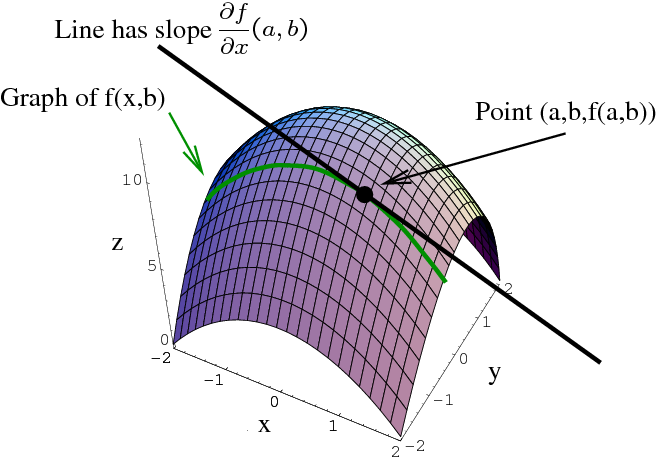
\includegraphics[scale=0.4]{3dpartial.png}
\end{frame}

%%%%%%%%%%%%%%
\begin{frame}{Example}
What are the critical points for
$$ f(x, y) = - (x^2 + y^2) $$
\end{frame}


%%%%%%%%%%%%%%
\begin{frame}{$ f(x, y) = - (x^2 + y^2)$}
\begin{center}
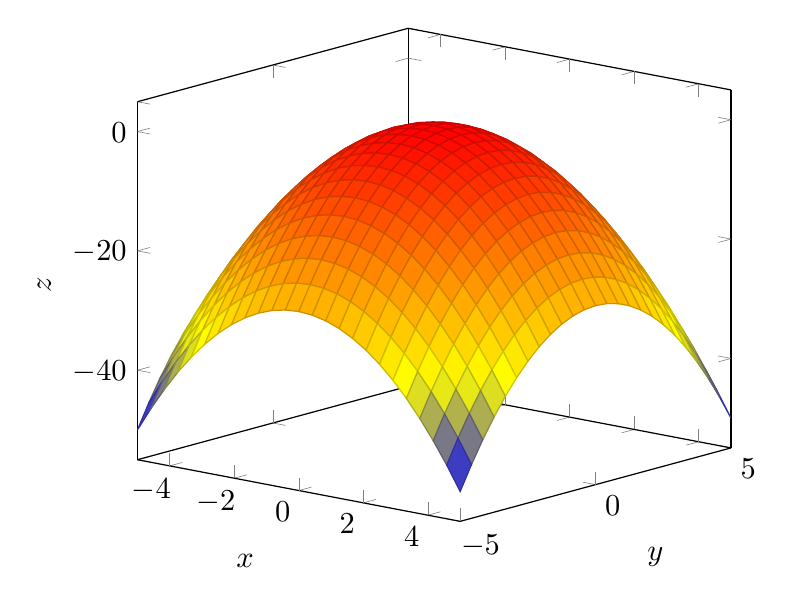
\begin{tikzpicture}[scale=1.1, transform shape]
\begin{axis}[view = {40}{15}, xlabel = \(x\), ylabel = \(y\), zlabel = \(z\)]
\addplot3 [surf] {-x^2 - y^2};
    \end{axis}
\end{tikzpicture}
\end{center}
\end{frame}

%%%%%%%%%%%%%%
\begin{frame}{Example}
What are the critical points for
$$ \pi(L, K) = f(K,L)- rK-wL $$
\end{frame}


%%%%%%%%%%%%%%
\begin{frame}{Second-Order Partial Derivatives}
For the function 
$$ z= f(x, y) $$ \\
$$
\begin{aligned}
f_{x x} & \equiv \frac{\partial}{\partial x} f_{x} \quad \text{ or } \quad \frac{\partial^{2} z}{\partial x^{2}} \equiv \frac{\partial}{\partial x}\left(\frac{\partial z}{\partial x}\right)  \\~\\
f_{y y} & \equiv \frac{\partial}{\partial y} f_{y} \quad \text{ or } \quad \frac{\partial^{2} z}{\partial y^{2}} \equiv \frac{\partial}{\partial y}\left(\frac{\partial z}{\partial y}\right)  \\
\end{aligned}
$$
\end{frame}

%%%%%%%%%%%%%%
\begin{frame}{Second-Order Partial Derivatives}
Also, have cross (or mixed) second-order partial derivatives.
$$
\begin{aligned}
f_{x y} & \equiv \frac{\partial^{2} z} {\partial x \partial y} &\equiv \frac{\partial}{\partial x}\left(\frac{\partial z}{\partial y}\right) \\~\\
f_{y x} & \equiv \frac{\partial^{2} z}{\partial y \partial x}  & \equiv \frac{\partial}{\partial y}\left(\frac{\partial z}{\partial x}\right) \\
\end{aligned}
$$
We always have  $f_{x y}=f_{yx}$ as long as $f_{x y}$ and $f_{y x}$ are both continuous. 
\end{frame}

%%%%%%%%%%%%%%
\begin{frame}{Example}
Find the four second-order partial derivatives of:
$$ z = x^3 + 5xy-y^2 $$
\end{frame}

%%%%%%%%%%%%%%
\begin{frame}{OLS}
\vspace{-1.5em}
$$ \min_{\{\alpha,\beta\}} \quad f(\alpha,\beta) = \sum_{i=1}^n (Y_i- \alpha - \beta X_i)^2  $$ \\~\\
First-order conditions:
\begin{align*}
	\frac{\partial f}{\partial \alpha} &= -2 \sum_{i=1}^n (Y_i- \alpha - \beta X_i) = 0 \\
	\frac{\partial f}{\partial \beta} &= -2 \sum_{i=1}^n (Y_i- \alpha - \beta X_i)X_i = 0
\end{align*}
\end{frame}


%%%%%%%%%%%%%%
\begin{frame}{Second-Order Condition}
Second-order (sufficient) conditions:\\~\\
For maximum:
 $f_{x x}<0, f_{y y}<0$, $f_{x x} f_{y y}>\left(f_{x y}\right)^{2}$. \\~\\
For minimum:
 $f_{x x}>0, f_{y y}>0$, $f_{x x} f_{y y}>\left(f_{x y}\right)^{2}$.
\end{frame}

%%%%%%%%%%%%%%
\begin{frame}{$ f(x, y) = - (x^2 + y^2)$}
\begin{center}
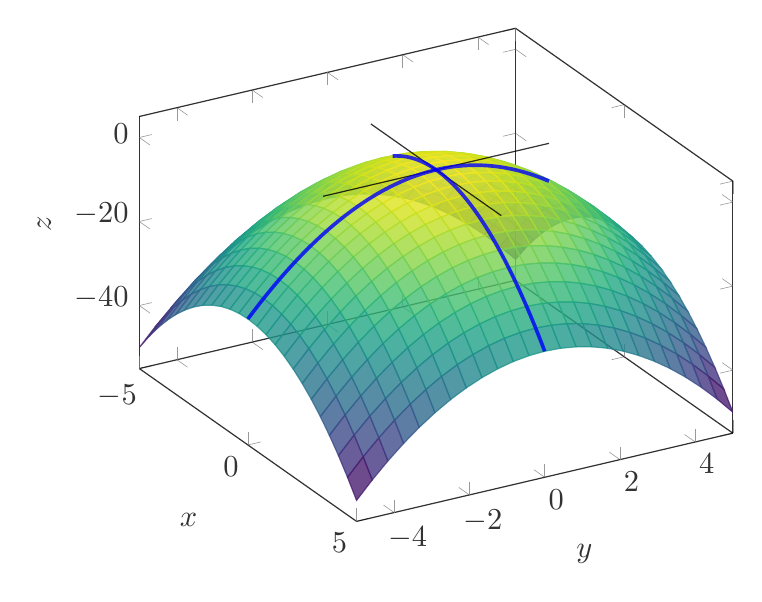
\begin{tikzpicture}[scale=1.1, transform shape, opacity=0.8]
\begin{axis}[view = {60}{35}, xlabel = \(x\), ylabel = \(y\), zlabel = \(z\)]
\addplot3 [surf, shader= flat, colormap/viridis, opacity=0.8, faceted color=black] {-x^2 - y^2};
\addplot3 [domain=-3:3, samples=50, samples y=0, black] (x, 0, 0); 
\addplot3 [domain=-3:3, samples=50, samples y=0, black] (0, x, 0); 
\addplot3 [domain=-2:5, samples=50, samples y=0, very thick, blue] (x, 0, -x^2); 
\addplot3 [domain=-5:3, samples=50, samples y=0, very thick, blue] (0, x, -x^2);  
\end{axis}
\end{tikzpicture}
\end{center}
\end{frame}

%%%%%%%%%%%%%%
\begin{frame}{$ f(x, y) = x^2 - y^2$}
\begin{center}
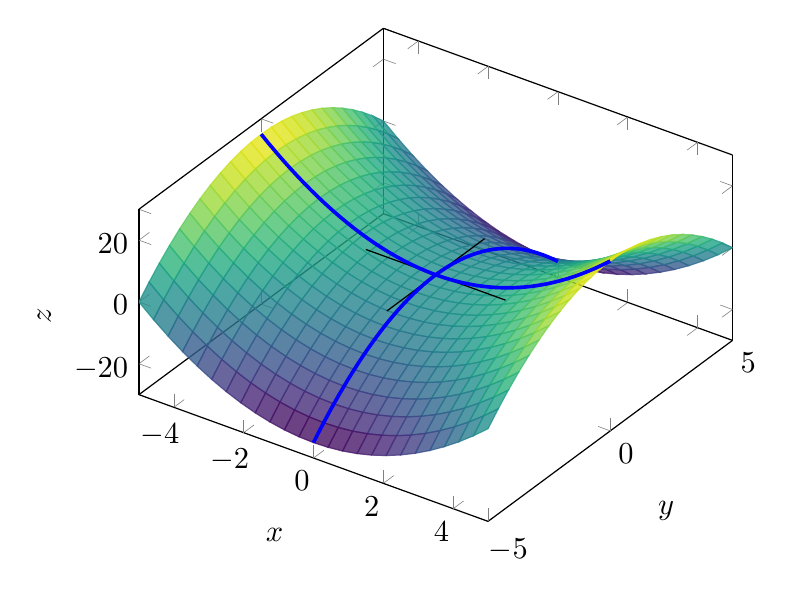
\begin{tikzpicture}[scale=1.1, transform shape]
\begin{axis}[view = {35}{50}, xlabel = \(x\), ylabel = \(y\), zlabel = \(z\)]
\addplot3 [surf, shader= flat, colormap/viridis, opacity=0.8, faceted color=black] {x^2 - y^2};
\addplot3 [domain=-2:2, samples=50, samples y=0, black] (x, 0, 0); 
\addplot3 [domain=-2:2, samples=50, samples y=0, black] (0, x, 0); 
\addplot3 [domain=-5:5, samples=50, samples y=0, very thick, blue] (x, 0, x^2); 
\addplot3 [domain=-5:5, samples=50, samples y=0, very thick, blue] (0, x, -x^2);  
\end{axis}
\end{tikzpicture}
\end{center}
\end{frame}

%%%%%%%%%%%%%%
\begin{frame}{$ f(x, y) = x^2 + y^2 + 5xy$}
\begin{center}
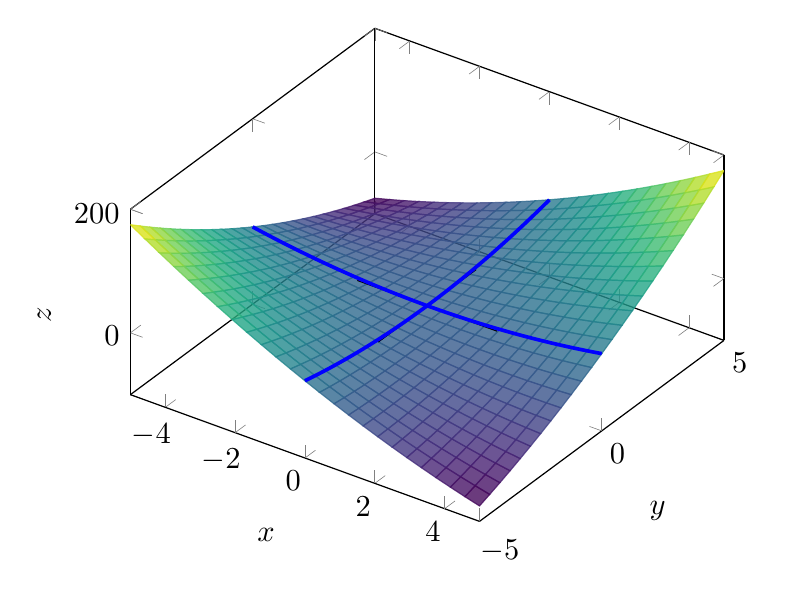
\begin{tikzpicture}[scale=1.1, transform shape]
\begin{axis}[view = {35}{50}, xlabel = \(x\), ylabel = \(y\), zlabel = \(z\)]
\addplot3 [surf, shader= flat, colormap/viridis, opacity=0.8, faceted color=black] {x^2 + y^2 + 5*x*y};
\addplot3 [domain=-2:2, samples=50, samples y=0, black] (x, 0, 0); 
\addplot3 [domain=-2:2, samples=50, samples y=0, black] (0, x, 0); 
\addplot3 [domain=-5:5, samples=50, samples y=0, very thick, blue] (x, 0, x^2); 
\addplot3 [domain=-5:5, samples=50, samples y=0, very thick, blue] (0, x, x^2);  
\end{axis}
\end{tikzpicture}
\end{center}
\end{frame}

\begin{frame}{Hessian Matrix}
For the function:
$$ y = f(x_1, x_2,...,x_n) $$
\vspace{0.25em}

The gradient vector $\nabla f$ and Hessian matrix $H$ is given by
$$ \nabla f = \begin{bmatrix}
	f_1 \\
	f_2 \\
	\vdots \\
	f_n
\end{bmatrix} \quad \quad
H = \begin{bmatrix}
	f_{11} & f_{12} & \hdots & f_{1n} \\
	f_{21} & f_{22} & \hdots & f_{2n} \\
	\vdots & \vdots & & \vdots \\
	f_{n1} & f_{n2} & \hdots & f_{nn} \\
\end{bmatrix} $$
\end{frame}

\begin{frame}{More than Two Choice Variables}
\vspace{1em}
\begin{tabularx}{\textwidth}{lXX}
\hline Condition & Maximum & Minimum \\
\hline \\ 
First-order & $f_1=f_2 =\hdots f_n=0$ & $f_1=f_2 =\hdots f_n=0$ \\
necessary & \text{i.e.} $\nabla f = 0$ & \text{i.e.} $\nabla f = 0$ \\~\\
Second-order  & $|H_1|<0, |H_2|>0,$ & $|H_1|, |H_2|, \hdots, |H_n|>0$ \\
sufficient & $|H_3|<0, \hdots$ & \\~\\
\hline
\end{tabularx}
\vspace{1em}

${ }^{\dagger}$ Applicable only after the first-order necessary condition has been satisfied.

\end{frame}


%%%%%%%%%%%%%%
\begin{frame}{References and Homework}
\begin{witemize}
  \item New sections today: Sections 11.1, 11.2
  \item Homework Problems: Exercise 11.2 1-5
  \item Reminder: Quiz 4 next week
\end{witemize}
\end{frame}





\end{document}